%
% Pull Down Resistor
%
\documentclass[border=3mm]{standalone}
\usepackage{tikz}
\usetikzlibrary{circuits.ee.IEC}

\begin{document}

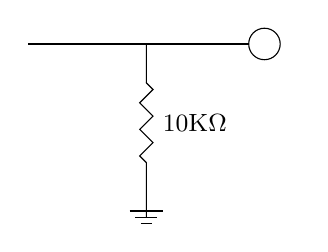
\begin{tikzpicture}[circuit ee IEC,small circuit symbols,
                    pin/.style={circle,draw=black!100,fill=white!20,thin, inner sep=0pt,minimum size=4mm}]
    \begin{scope}[set resistor graphic=var resistor IEC graphic,
                  set diode graphic=var diode IEC graphic,font=\small]
        \node (output) at (3,0) [pin,label=right: ] {};
        \draw [-] (0,0) to (output);
        \draw (1.5,0) to [resistor={ohm=10K},point down] (2,1.5)
                      to (1.5,-2.2) node [ground,point down] {} (1.5,-2.2);
    \end{scope}
\end{tikzpicture}

\end{document}

